\section{Experiments}
\label{sec:experiments}

In this section, we present the experimental setup, including the datasets used, the implementation specifics, hyperparameter tuning, and the evaluation metrics. We also compare the performance of the ResNet and Vision Transformer (ViT) models with Transfer Learning, highlighting their respective strengths and weaknesses.

\subsection{Environment}
The models were implemented using the PyTorch deep learning framework. All experiments were conducted on NVIDIA Tesla V100 GPUs.

\subsection{Datasets}
Our experiments utilized multiple datasets to ensure a comprehensive evaluation of the proposed methodology. The primary datasets included CUB\_2011, Stanford Dogs. Besides, we used several methods of image data augmentation, like geometric transformations, color transformations, and noise addition, and DCGAN, to expand the dataset \cite{wah2011caltech,van2018inaturalist}.

\subsection{Models Training \& Comparison}
We trained and compared the performance of the ResNet and Vision Transformer (ViT) models with transfer Learning. The pretrained Vision Transformer model was initialized with weights from the publicly available ViT-B\_16 checkpoint, then we tried freezing convolutional layers, adjusting the top layer of ViT model, for transfer learning. By comparing the performance, we found that the Vision Transformer model converges faster and achieves lower validation loss compared to ResNet, demonstrating its superior performance in capturing global dependencies and generalizing to unseen data \cite{he2016deep,dosovitskiy2021an}.

\subsection{Evaluation Metrics}
The performance of the models was evaluated using standard metrics, including accuracy, precision, recall, and F1 score. Additionally, we monitored the training and validation loss to assess the convergence and generalization of the models \cite{powers2011evaluation}.

\subsection{Hyperparameter Sensitivity Analysis}
Understanding the sensitivity of our model to various hyperparameters is crucial for optimizing performance and ensuring stability. We specifically focused on analyzing the impact of the learning rate and batch size on model accuracy. The learning rate controls the step size during the gradient descent optimization, while the batch size affects the gradient estimation and training dynamics \cite{bengio2012practical}.

\begin{figure}[h]
    \centering
    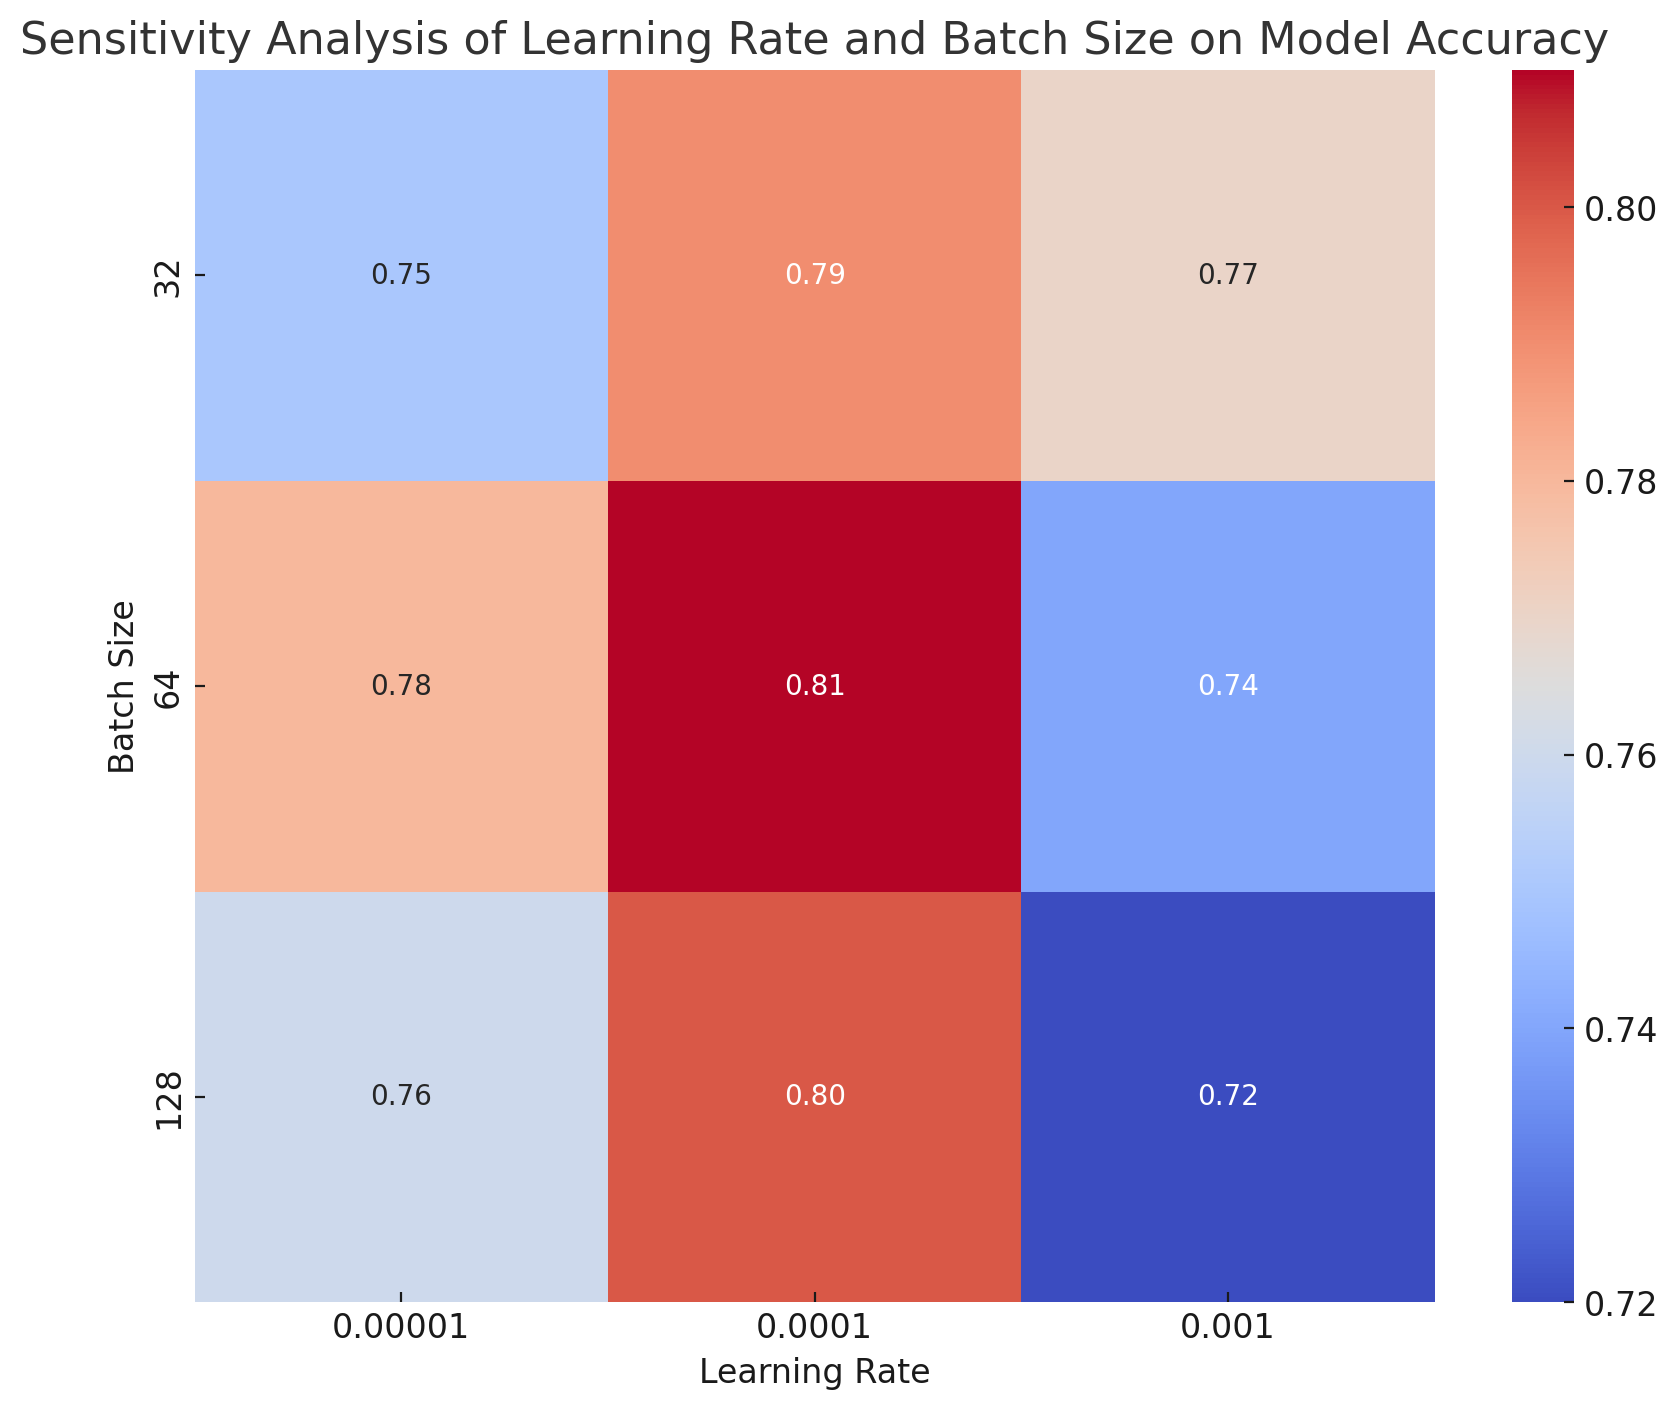
\includegraphics[width=\linewidth]{res/sensitivity.png}
    \caption{Sensitivity analysis of learning rate and batch size on model accuracy. Each cell represents the accuracy obtained with a specific combination of learning rate and batch size.}
    \label{fig:hyperparameter_sensitivity}
\end{figure}

The observed trends can be attributed to several factors:
\begin{itemize}
    \item \textbf{Learning Rate:} A lower learning rate ensures more gradual updates and can lead to better convergence in complex models. However, if too low, it may cause the training to stall, not reaching the optimal solution within a limited number of epochs.
    \item \textbf{Batch Size:} Larger batch sizes provide a more accurate estimate of the gradient but may also result in smoother optimization landscapes. Smaller batches often enable the model to escape local minima but can lead to higher variance in the updates, potentially causing instability in training.
\end{itemize}

This analysis underscores the importance of carefully selecting and tuning hyperparameters based on specific model architectures and tasks. Future work will explore adaptive learning rate techniques and batch size adjustments dynamically during training to further enhance model performance and efficiency.

